\chapter{绪论}

\label{chap:intro}
\section{研究背景和意义}

近年来，大语言模型（Large Language Models, LLMs）在自然语言理解与生成领域取得了突破性进展。凭借海量语料预训练和大规模参数建模能力，LLM 已经在问答、对话生成、文本摘要、信息抽取、逻辑推理等多类任务中表现出优异性能，并逐步成为新一代通用人工智能系统的重要基础设施\cite{DBLP:conf/nips/BrownMRSKDNSSAA20,DBLP:journals/corr/abs-2108-07258,DBLP:conf/nips/KojimaGRMI22}。有研究指出，LLM 的兴起改变了传统面向单任务训练专用模型的开发范式，使研究者和开发者能够基于统一的基础模型完成多种下游任务，从而显著提升了语言技术的适应性与通用性\cite{DBLP:journals/coling/GallegosRBTKDYZA24}。

然而，LLM 在展现强大能力的同时，也暴露出明显的社会偏见问题。由于模型通常依赖大规模互联网语料进行训练，而这些语料本身包含历史与现实社会中的偏见、刻板印象、歧视性表达等语言文字，模型在学习语言模式的过程中也会一定程度继承和保留这些偏见，甚至放大这些有害倾向\cite{DBLP:conf/fat/BenderGMS21,DBLP:conf/emnlp/DodgeSMAIGM021,DBLP:conf/acl/ShengCNP20}。LLM 的偏见并不只表现为显式冒犯或仇恨性语言回复，还包括由于刻板印象而造成面向不同群体的不一致输出等多种形式，这些问题会对处于弱势或边缘地位的社会群体造成更为明显的负面影响。

随着 LLM 被广泛应用到招聘辅助、教育咨询、医疗问答、内容审核、智能推荐等与社会公平密切相关的场景中，其偏见问题已经不仅是模型性能缺陷，更是影响系统可信性、用户体验与社会公正的重要因素。这意味着，LLM 偏见问题不仅涉及技术层面的鲁棒性与可控性，也直接关系到人工智能系统的伦理安全与可持续部署\cite{DBLP:journals/firstmonday/Ferrara23a}。

现有研究围绕大语言模型偏见问题已形成一定的技术基础，相关工作主要集中在公平性评测、偏见检测和偏见缓解三个方面。公平性评测方法主要借助评测指标与测试数据集，从整体上分析模型在不同敏感属性条件下是否存在系统性输出差异。偏见检测方法则进一步面向具体输入输出实例，借助反事实构造、分类器或裁判模型识别偏见是否发生以及偏见表现于何处。偏见缓解方法则通过预处理、训练中、推理中和后处理等手段削弱模型生成内容中的不公平倾向。现有方法虽然能够在一定程度上提升模型公平性，但仍普遍存在修改粒度较粗、语义漂移明显、信息保留不足和过度拒答等问题，难以兼顾公平性改善与回复质量。尤其是在当前主流大语言模型多以 API 或在线服务形式部署、模型参数与训练细节不可见的背景下，传统依赖再训练、参数更新或内部表示干预的方法适用性受到明显限制。

基于此，围绕黑盒场景下的大语言模型偏见识别与输出级校正开展研究具有重要意义。在方法层面，可为黑盒条件下的实例级偏见定位、风险量化与最小编辑校正提供新思路。在应用层面，有助于提升大语言模型在真实场景中的公平性、可信度与可部署性，为构建更安全、更负责任的智能系统提供技术支撑。


\section{国内外研究现状}

围绕大语言模型公平性的研究，国内外学者已从公平性概念建模、偏见评测、偏见检测、偏见缓解以及配套评测资源构建等多个方向展开探索，逐步形成了较为系统的研究脉络。现有工作一方面借鉴机器学习公平性研究中关于群体公平性与个体公平性的基本思想，并将其扩展到大语言模型的表示、概率与生成行为分析中；另一方面，则围绕模型偏见的发现、量化与干预，发展出从评测到检测、再到缓解的多层次技术路径。图~\ref{fig:llm-fairness-framework} 对相关研究进行了归纳展示。基于本文的研究重点，下面将从大语言模型公平性评测、偏见检测以及偏见缓解与输出重写三个方面，对国内外研究现状进行梳理。

\begin{figure}[htbp]
    \centering
    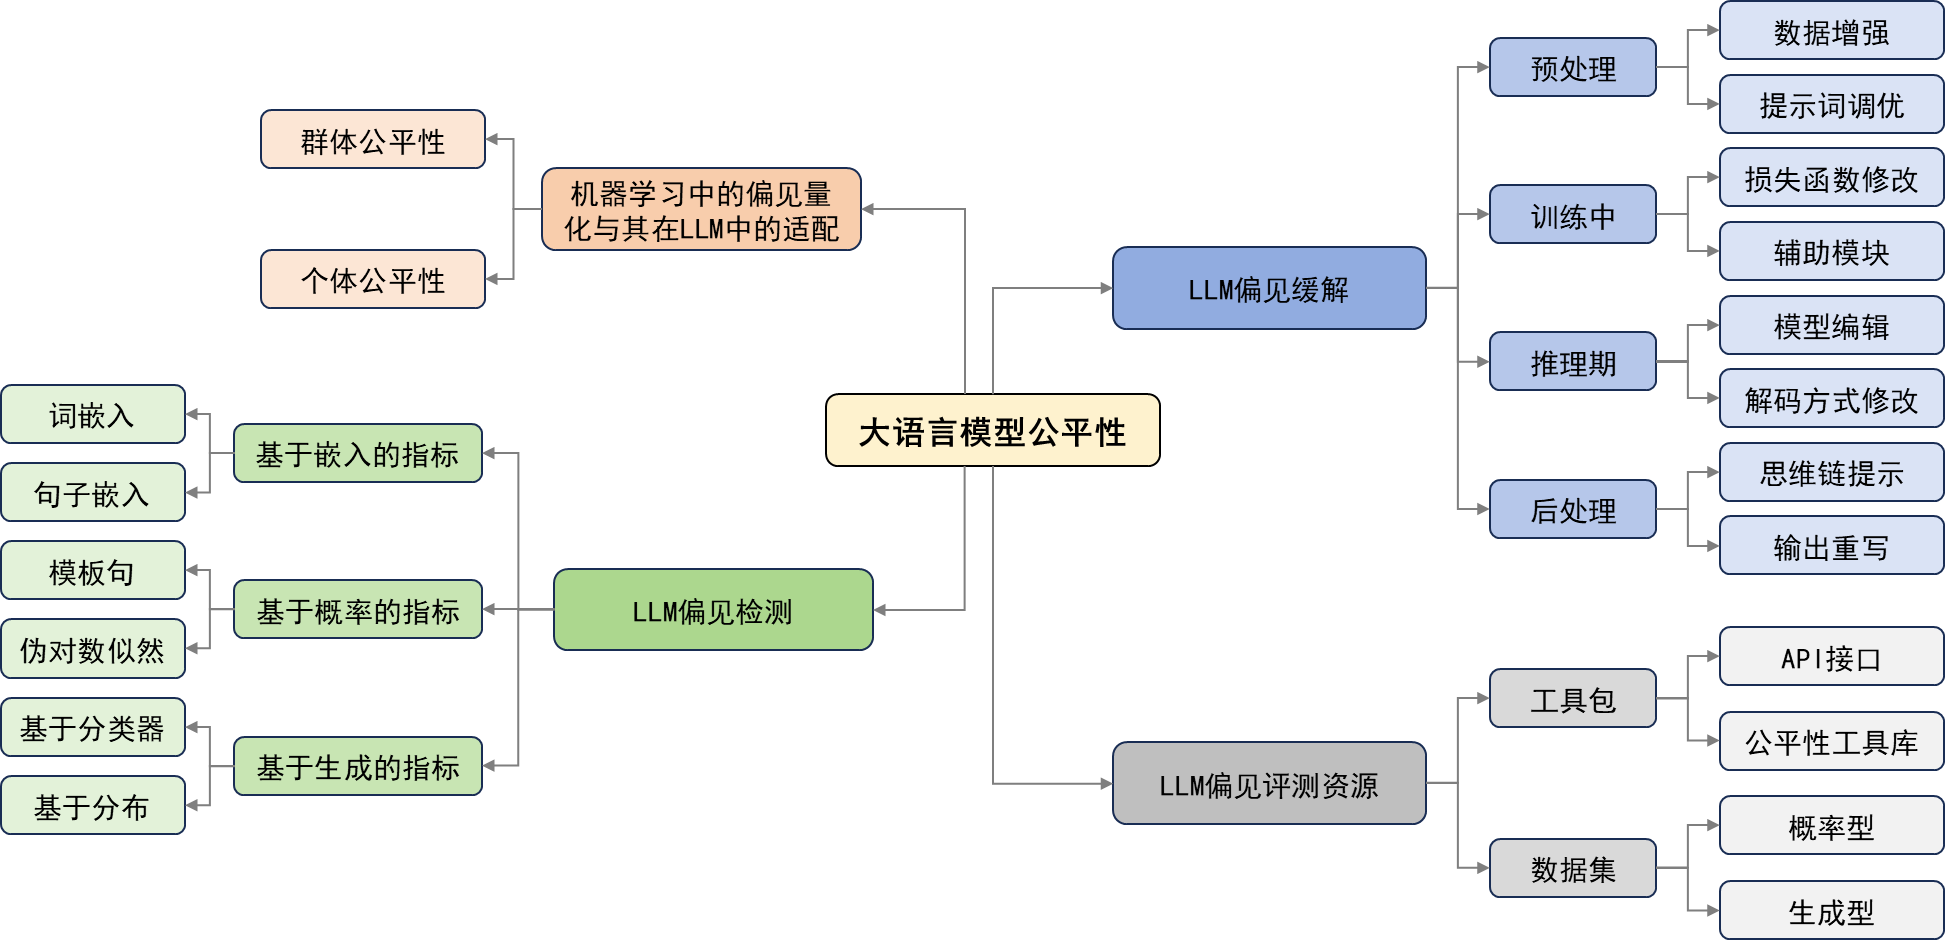
\includegraphics[width=1.0\textwidth]{figures/chap1/大语言模型公平性研究分类框架.png}
    \caption{大语言模型公平性研究分类框架}
    \label{fig:llm-fairness-framework}
\end{figure}

\subsection{大语言模型公平性评测研究现状}

大语言模型公平性评测的核心目标是系统测量模型在涉及不同敏感属性时的输出差异，从而判断模型是否存在不公平行为。随着词向量和预训练语言模型的发展，研究者首先从表示空间中的群体关联关系入手，对模型是否学习到性别、种族等社会属性的刻板关联进行分析。Caliskan等人\cite{DBLP:journals/corr/IslamBN16}提出 WEAT 方法，通过比较社会群体词与中性属性词在嵌入空间中的距离关系来刻画偏见。May等人\cite{DBLP:conf/naacl/MayWBBR19}提出 SEAT 方法，将该思想扩展到上下文化句子表示。Tan等人\cite{DBLP:conf/nips/TanC19}进一步比较不同社会群体词在具体句子语境中的表示差异，用于分析上下文条件下是否仍存在稳定的群体刻板关联。Guo等人\cite{DBLP:conf/aies/GuoC21}提出 CEAT 方法，通过对多次采样得到的偏见效应进行统计汇总，减少单一模板或单次表示提取带来的偶然性，从而提高上下文化偏见评测的稳健性。Dolci等人\cite{DBLP:journals/dase/DolciAT23}则提出句子偏差评分方法，不再只看整句的整体表示，而是进一步分析句子中各个词对性别偏向的贡献强弱。此类研究为理解偏见在模型表征层面的存在形式提供了基础，但后续研究也表明，嵌入空间中的偏差与下游任务中的真实不公平并不总能稳定对应，且评测结果容易受模板构造、种子词选择和表示提取方式的影响\cite{DBLP:conf/acl/Goldfarb-Tarrant20,DBLP:conf/naacl/DelobelleTCB22,DBLP:conf/fat/CabelloJS23}。

在表示层评测基础上，研究逐步发展出基于模型概率的公平性评测方法。这类方法通常通过替换敏感属性、构造成对句子或模板输入，比较模型在不同群体条件下对词或句子的概率分配差异。Kurita等人\cite{DBLP:journals/corr/abs-1906-07337}提出对数概率偏差评分，通过归一化 token 概率测量职业等中性属性与群体词之间的偏好差异。Webster 等人\cite{DBLP:journals/corr/abs-2010-06032}提出 DisCo，通过填空模板比较不同群体触发下模型预测结果的分布差异。Ahn等人\cite{DBLP:conf/emnlp/AhnO21}进一步将归一化对数概率扩展到非二元目标群体。Nangia等人\cite{DBLP:conf/emnlp/NangiaVBB20}提出 CrowS-Pairs 及其对应的伪似然打分方法，用于比较 stereotype 与 anti-stereotype 句子的相对偏好。Nadeem等人\cite{DBLP:conf/acl/NadeemBR20}构建 StereoSet 数据集，并提出 CAT 与 iCAT 指标，同时考察句内和句间的刻板印象偏好。Kaneko等人\cite{DBLP:conf/aaai/KanekoB22}提出 AUL 与 AULA，试图减少掩码选择带来的测量偏差。Barikeri等人\cite{DBLP:conf/acl/BarikeriLVG20} 则以困惑度差异为基础提出语言模型偏差。相较于表示层方法，概率类方法更直接反映模型在特定输入条件下的偏好，但其对模板和句对构造依赖较强，并且“应该用相等概率对待 stereotype 与 anti-stereotype的公平性假设本身存在争议”，因而在复杂场景中的解释力仍受限制\cite{DBLP:conf/acl/BlodgettLOSW20,DBLP:conf/pkdd/DelobelleB22,DBLP:conf/coling/KanekoBO22}。

随着生成式大语言模型成为主流，公平性评测进一步转向基于生成文本的输出行为分析。与表示或概率方法不同，这类方法直接利用模型生成的自然语言文本进行偏见评估，特别适用于闭源或 API 形式提供服务的黑盒模型。Sheng等人\cite{DBLP:conf/emnlp/ShengCNP19}较早利用前缀提示与 regard 分类器分析模型对不同社会群体的社会评价倾向。Gehman等人\cite{DBLP:conf/emnlp/GehmanGSCS20}提出 RealToxicityPrompts 数据集，通过向模型输入真实网络文本前缀，统计生成结果中最大毒性、毒性概率和毒性比例等指标，评估模型在开放生成场景中的有害输出风险。Dhamala\cite{DBLP:conf/fat/DhamalaSKKPCG21}构建 BOLD 数据集，结合心理语言学规范指标分析不同群体相关提示下模型的生成差异。Nozza等人\cite{DBLP:conf/naacl/NozzaBH21}提出 HONEST，采用词典匹配方式检测生成结果中的伤害性补全内容。
% Liang等人\cite{liang2022helm}从词语共现分布和人口群体表征两个角度提出 Demographic Representation 与 Stereotypical Associations 指标。
Sicilia等人\cite{DBLP:conf/acl/SiciliaA23}、Huang等人\cite{DBLP:conf/emnlp/HuangZJSWRMYK20} 以及 Smith等人\cite{DBLP:conf/emnlp/SmithHKPW22}分别从群体间评分是否一致、反事实替换后的情感变化，以及完整生成文本在不同群体提示下的波动程度等方面，对生成式偏见进行了分析。与此同时，Parrish等人\cite{DBLP:conf/acl/ParrishCNPPTHB22}提出 BBQ 数据集，将偏见评测引入问答任务。Li等人\cite{DBLP:journals/corr/abs-2010-02428}提出的 UnQover、Krieg等人\cite{DBLP:conf/chiir/KriegPMLSR23}提出的 Grep-BiasIR 也分别将评测扩展到问答与检索场景。

总体来看，公平性评测研究已从表示层关联分析发展到概率比较，再到基于开放生成和真实任务输出，形成了较为完善的指标体系与测试数据集资源。然而，公平性评测的重点主要在于判断模型是否存在偏见以及不同模型之间的表现差异，对于如何在具体实例中进一步识别偏见来源、定位偏见表现并为后续修正提供依据的关注仍相对不足。基于此，研究者开始在公平性评测之外进一步发展面向实例识别的偏见检测方法。

\subsection{偏见检测方法研究现状}

早期偏见检测方法大多沿用评测框架中的模板化替换思路，通过显式敏感属性扰动来比较模型在不同社会群体条件下的响应差异。例如，Rudinger等人\cite{DBLP:conf/naacl/RudingerNLD18} 提出的 Winogender、Zhao等人\cite{DBLP:conf/naacl/ZhaoWYOC18} 提出的 WinoBias、Vanmassenhove等人\cite{DBLP:conf/emnlp/VanmassenhoveES21} 提出的 WinoBias+、Webster等人\cite{DBLP:journals/tacl/WebsterRAB18} 提出的 GAP、Levy等人\cite{DBLP:conf/emnlp/LevyLS21} 提出的 BUG 等，主要通过代词消解和职业和性别匹配任务检测模型是否依赖刻板印象。这类方法在检测显式性别偏见和职业刻板印象方面较为有效，但更多针对结构化模板和受限句式，难以应对开放自然语言输入中的隐式敏感属性与复杂语义。

随后，基于反事实输入或句对比较的检测方法成为偏见识别的核心路线。Nangia等人\cite{DBLP:conf/emnlp/NangiaVBB20} 提出的 CrowS-Pairs、Barikeri等人\cite{DBLP:conf/acl/BarikeriLVG20} 提出的 RedditBias、Felkner等人\cite{DBLP:conf/acl/FelknerCJM23} 提出的 WinoQueer、Qian等人\cite{DBLP:conf/emnlp/QianRFSKW22} 提出的 PANDA、Dev等人\cite{DBLP:conf/aaai/DevLPS20} 提出的 Bias NLI 等，都通过对社会群体描述进行替换、保持句子语义主干基本一致的方式，检测模型在不同群体条件下的判断或生成差异。该类方法的重要优势在于，其能够较自然地体现“如果仅改变敏感属性，模型输出是否应保持一致”这一公平性要求，因此在理论上与个体公平、反事实公平等理念具有较强关联\cite{DBLP:conf/innovations/DworkHPRZ12,DBLP:journals/csur/MehrabiMSLG21}。然而，Blodgett等人\cite{DBLP:conf/acl/BlodgettLOSW20}指出，许多现有反事实基准中的刻板印象与反刻板印象句对在现实权力关系表达上并不总是合理，部分样本甚至无法明确刻画真实世界中的偏见结构。Selvam等人\cite{DBLP:conf/acl/SelvamDKKC23}进一步表明，一些表面微小的词汇改动就可能显著影响偏见得分。这说明反事实检测虽然具有较强的可解释性，但其有效性高度依赖于敏感属性替换是否自然、语义是否真正保持一致，以及差异是否确实由偏见而非任务语义变化导致。

从研究脉络来看，偏见检测的价值不仅在于识别模型是否存在问题，更在于为后续干预提供依据。只有当研究者能够较为稳定地判断偏见是否发生、由何种敏感属性触发以及偏见主要体现于哪些内容时，偏见缓解方法才能进一步针对模型训练过程、推理行为或最终输出开展有针对性的修正。

\subsection{偏见缓解方法研究现状}

偏见缓解技术与偏见评测和检测并行发展，现有缓解方法大致沿着预处理、训练中、推理中和后处理四个阶段逐步演进。预处理方法主要通过数据增强、数据过滤、重加权、数据生成和指令调控等方式，在模型训练之前减少训练语料中的群体偏差。
其中，一类研究通过反事实数据增强或替代策略来平衡不同社会群体的样本分布 \cite{DBLP:conf/birthday/LuMWAD20,DBLP:conf/emnlp/MaudslayGCT19,DBLP:conf/acl/GhanbarzadehHPM23}。
另一类研究则借助样本筛选、毒性清洗和重加权等手段，降低训练数据中的偏见负担 \cite{DBLP:conf/aies/DixonLSTV18,DBLP:conf/ijcnlp/GarimellaMA22,DBLP:journals/corr/abs-2205-11374,DBLP:conf/acl/ThakurJVLM23,DBLP:journals/corr/abs-2108-07790,DBLP:conf/nips/SattigeriGPDV22}。
还有一些工作从示范样本构建、社会规范数据补充以及人类反馈数据生成等角度出发，进一步改进训练语料 \cite{DBLP:conf/emnlp/DinanFWUKW20, DBLP:conf/nips/SolaimanD21, DBLP:conf/emnlp/0002YJLKKCS22, DBLP:conf/acl/UngXB22, DBLP:conf/acl/0012ZMWLCW0H23}。
此外，也有研究通过指令设计、触发词或连续提示等方式优化模型输入 \cite{DBLP:journals/corr/abs-2212-10678, DBLP:conf/eacl/VenkitGPHW23, DBLP:conf/aies/AbidF021, DBLP:conf/acl/FatemiXLX23}。
此类方法可在一定程度上提升整体公平性，但依赖有效的社会群体词表、人工规则或再训练过程，且容易引入语法错误、事实偏移或新的分布失衡 \cite{DBLP:conf/eacl/KumarBNAT23, DBLP:conf/fat/DevinneyBB22}。

训练阶段的偏见缓解则更加关注模型内部参数和目标函数的调整。为削弱社会群体与特定语义之间的耦合关系，研究者提出了多种正则化、对抗学习和强化学习方法。\\
部分研究从表示学习层面入手，尝试通过表示子空间约束、正交约束以及互信息最小化等方法削弱模型对敏感属性的编码 \cite{DBLP:conf/naacl/BordiaB19, DBLP:conf/acl/RavfogelEGTG20, DBLP:conf/acl/LiangLZLSM20, DBLP:conf/icassp/WooNJL23}。
在此基础上，Guo等人 \cite{DBLP:conf/acl/GuoYA22} 通过对输出分布、logits 以及偏见词能量施加正则约束，实现了对生成行为的公平控制。随后，Gaci等人 \cite{DBLP:conf/emnlp/GaciBCB22} 将去偏目标进一步融入注意力分布的调整过程，Zheng等人 \cite{DBLP:conf/acl/ZhengK0H23} 借助对比学习提升偏见对照样本表征的一致性，Jin等人 \cite{DBLP:conf/naacl/JinBKDNR21} 则通过强化学习或价值对齐策略将公平性目标纳入奖励函数。总体来看，这类方法在开放模型中具有较强的控制能力，但通常依赖于对模型内部参数或训练过程的访问，因此难以直接适用于当前大量仅以 API 形式提供能力的黑盒大语言模型。

在无法直接训练或修改模型的场景下，研究进一步转向推理阶段和后处理阶段的去偏方法。推理阶段方法主要通过改写解码过程来约束模型输出，例如Xu等人\cite{DBLP:journals/corr/abs-2010-07079}利用敏感词或 n-gram 阻断减少有害生成。Shuster等人\cite{DBLP:journals/corr/abs-2208-03188}和Schramowski等人\cite{DBLP:journals/natmi/SchramowskiTARK22}通过分类器或价值判断器重新排序生成候选。Saunders等人\cite{DBLP:conf/acl/SaundersSB22}和Meade等人\cite{DBLP:conf/emnlp/MeadeGHGJRLH23}利用约束搜索、逻辑约束或安全示例引导生成更公平的输出。Krause等人\cite{DBLP:conf/emnlp/KrauseGMKJSR21}和Liu等人\cite{DBLP:conf/acl/LiuKW23}则通过专家—反专家模型、自我去偏或偏置项重分配修改 token 概率分布。Zayed等人\cite{DBLP:journals/corr/abs-2305-13088} 和 Hauzenberger等人\cite{DBLP:conf/acl/HauzenbergerMKS23} 从注意力重分布和模块化去偏网络角度提供无需完整再训练的中间方案。这些方法比训练阶段技术更灵活，但仍常要求访问 logits、注意力权重或中间表示，且过强的解码约束可能影响输出多样性和可用性，甚至压制少数群体语言表达。

真正最贴近黑盒大语言模型应用现实的，是后处理阶段的输出重写方法，这类方法直接修改模型生成文本，而不依赖访问内部参数，是黑盒场景下重要的偏见缓解路径。Pryzant等人\cite{DBLP:conf/aaai/PryzantMDKJY20} 较早构建平行语料，将带有主观偏差的句子重写为更中性的表达。Ma等人\cite{DBLP:conf/emnlp/MaSRC20}尝试从权力关系和能动性角度对句子进行神经改写。He等人\cite{DBLP:conf/emnlp/HeMM21}首先识别受保护属性词，再通过神经重写模型生成去偏文本。Dhingra等人\cite{DBLP:journals/corr/abs-2307-00101} 对敏感属性相关刻板表达进行解释和替换，并通过风格迁移保持原句语义。Amrhein等人\cite{DBLP:conf/acl/AmrheinSSL23}将偏见修正建模为机器翻译式重写任务，在平行的偏见和去偏文本上训练生成模型。Majumder等人\cite{DBLP:conf/emnlp/MajumderHM23}提出 InterFair，在用户可控条件下调整重写强度。此类方法表明，输出级重写可以在不干预底层模型的前提下有效削弱偏见，是黑盒模型公平校正的可行方向。

\subsection{现有研究存在的问题}

综上所述，现有研究虽然已经在大语言模型偏见评测、检测与缓解方面取得了较多进展，但与黑盒大语言模型输出公平性治理的实际需求相比，仍存在以下三个方面的突出问题。

1. 黑盒条件下缺少稳定的偏见识别路径。现有许多方法依赖模型内部表示或训练过程，难以直接迁移到以 API 形式提供服务的黑盒大语言模型。能够在黑盒场景中使用的方法，大多依赖单次判断、规则匹配或表面词汇统计，难以有效识别隐式偏见和语义层面的差别对待。如何仅基于输入输出行为构造可比较、可解释的偏见识别过程，仍然是当前研究中的核心难点。

2. 输出差异与真实偏见之间缺少高置信验证机制。在黑盒生成场景中，原始回复与反事实回复之间出现差异，并不必然意味着模型存在偏见，该差异也可能来自任务语义本身的合理变化、事实条件不同或生成模型的随机波动。现有研究对由敏感属性变化触发的不合理差异和由事实或语义差异导致的合理变化区分不足，容易产生误判或过度公平判断。

3. 输出级偏见校正缺少细粒度、可控的局部重写机制。现有后处理方法虽然表明输出重写是黑盒场景下可行的偏见缓解路径，但不少方法仍以整体改写为主，容易带来信息丢失、语义漂移、回复可用性下降等副作用。

以上问题构成了本文研究的背景，也对应了本文围绕反事实偏见识别、高置信偏见验证和最小编辑偏见重写的三项核心研究内容。


\section{本文研究内容}

本文围绕黑盒大语言模型输出偏见的识别与校正问题展开研究。针对当前大量大语言模型以 API 或封闭服务形式提供能力的现实应用场景，本文从输出行为分析出发，将反事实公平思想、差异检测方法与输出后处理策略结合，构建了一个模型偏见回复识别与重写的算法框架。具体研究内容包含以下三个部分。

1. 提出一种面向黑盒大语言模型的基于反事实输入构造的偏见识别方法。针对黑盒条件下难以访问模型内部参数、传统表示层或概率层方法难以直接适用的问题，本文首先从输入层出发，对敏感属性进行识别、统一表征与替换，构造语义主干保持一致的原始 prompt 与反事实 prompt 对。通过比较原始回复与反事实回复在语义偏移、态度变化和生成偏好上的差异，建立候选偏见分数计算模型。该方法将反事实公平思想引入黑盒输出级偏见检测过程，为 API 形式大语言模型提供了一条无需访问模型内部结构的偏见识别路径。

2. 提出一种融合公平性与事实性的高置信偏见验证机制。针对单纯依赖差异分数容易将任务语义变化、生成波动或合理事实差异误判为偏见的问题，本文在候选偏见回复基础上，进一步设计二阶段验证流程。该流程先从原始回复与反事实回复中抽取差异命题，再结合基于 CoT 的反思式判定链，从事实性与公平性两个角度对差异进行再判断，得到最终偏见风险分数和偏见标签。该机制提升了偏见识别结果的高置信度和可解释性，也为后续偏见校正提供了更可靠的输入基础。

3. 提出一种基于高风险片段定位与最小编辑约束的偏见重写方法。针对现有整体重写方法修改范围过大、易造成信息丢失和语义漂移的问题，本文在重写阶段进一步设计了输出级偏见校正框架。首先对偏见回复进行高风险片段定位，并结合片段偏见风险、重写代价和综合优先级确定最终重写单元。然后在最小编辑约束、内容保持约束以及长度与结构约束下执行局部定向重写，并通过信息保留度校验、语义连贯性校验和新风险引入检测实现重写结果的接受与回退。该方法实现了片段级偏见校正，为黑盒大语言模型输出后处理提供了更细粒度、可控性更强的技术方案。

\section{本文组织结构}

本文围绕黑盒大语言模型输出偏见的识别、验证与重写问题展开研究，针对当前黑盒条件下偏见识别困难、识别结果与校正过程脱节以及输出级校正缺少细粒度可控机制等关键问题，提出了基于反事实检测与约束重写的偏见修正方法。围绕上述研究目标，本文从相关理论与技术分析出发，依次开展黑盒条件下的偏见识别方法研究、高风险偏见片段定位与最小编辑重写方法研究，并通过实验对所提方法的有效性进行系统验证。本文整体结构如图~\ref{fig:framework}，论文全文共分为五章，各章节内容安排如下。

\begin{figure}[htbp]
    \centering
    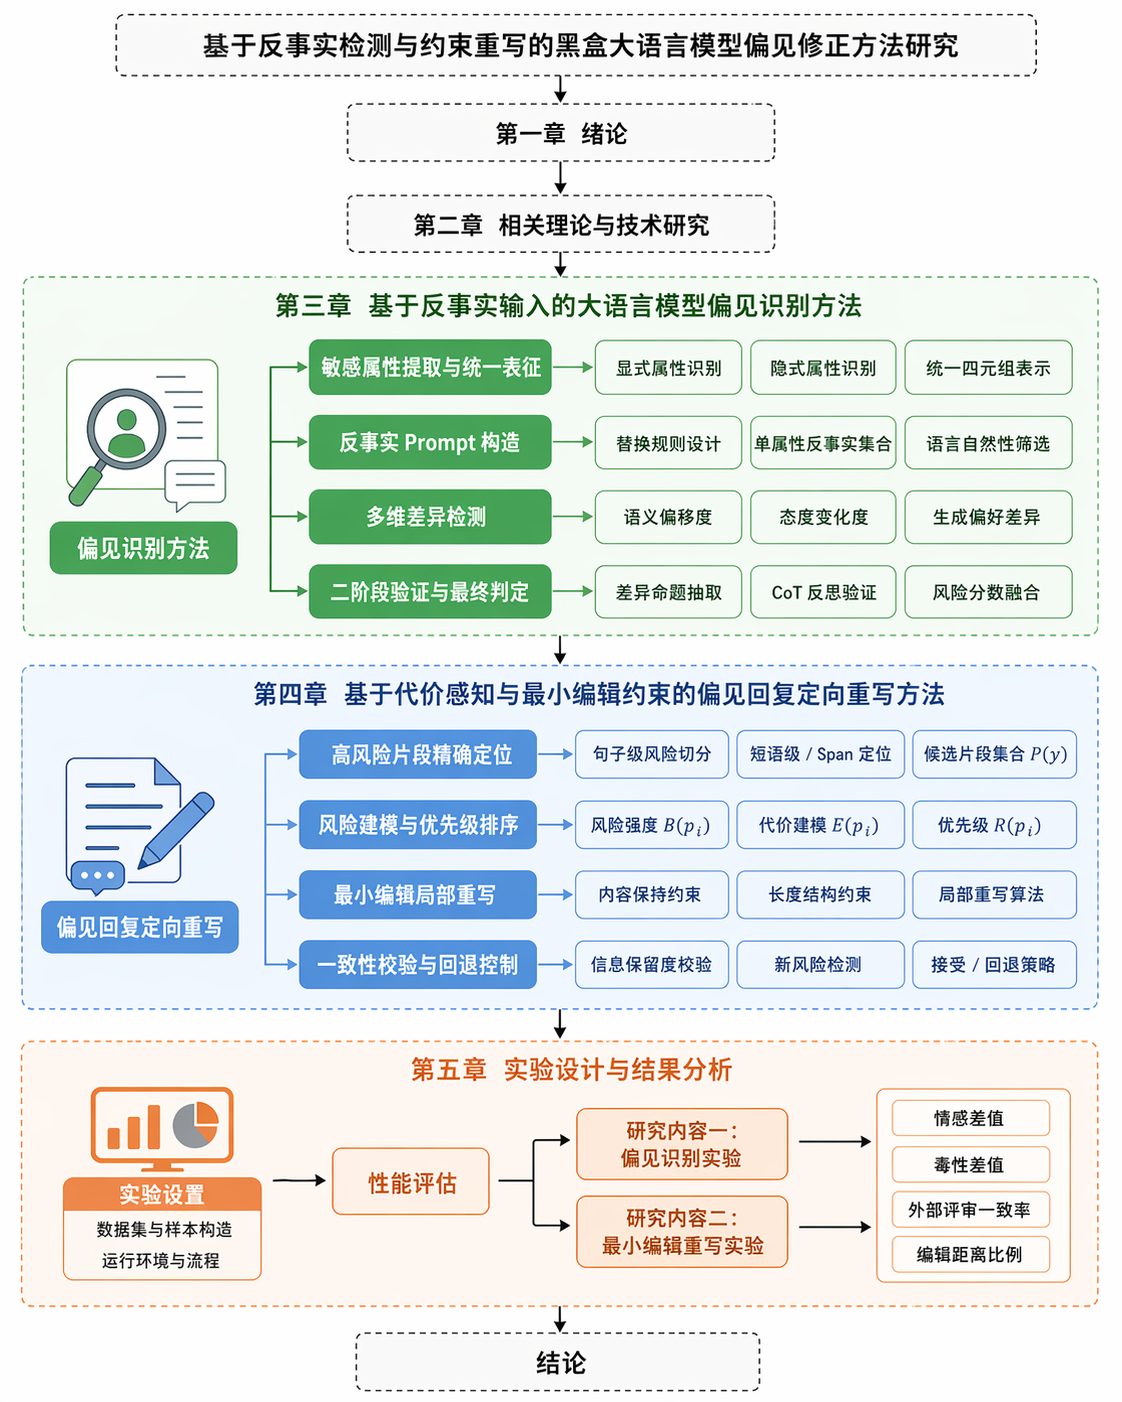
\includegraphics[width=1.0\textwidth]{figures/chap1/文章组织架构图.png}
    \caption{本文的组织安排}
    \label{fig:framework}
\end{figure}

第一章，绪论。本章首先介绍本文的研究背景与研究意义，分析黑盒大语言模型输出偏见问题的现实挑战和研究价值。随后，介绍国内外在大语言模型公平性评测、偏见检测与偏见缓解等方面的研究现状，进一步提出本文拟解决的关键问题，并概述本文的研究内容、创新点及整体组织结构。

第二章，相关理论与技术研究。本章围绕本文后续方法设计所需的理论基础与关键技术展开介绍。首先阐述大语言模型偏见与公平性的基本概念、偏见来源及公平性判别准则。然后，系统分析偏见评测任务的形式化定义、基于表示空间、条件概率和生成文本的评测方法，以及偏见评测数据与资源的技术组织方式。最后对偏见缓解与输出重写技术、反事实公平性分析思想及其在黑盒场景中的适用性进行总结，为后续方法设计奠定理论基础。

第三章，基于反事实替代检测的大语言模型输出偏见识别方法。本章针对黑盒条件下难以利用模型内部信息进行偏见检测的问题，首先给出偏见检测任务定义与总体方法框架。然后，研究敏感属性识别、统一表征与反事实 prompt 构造方法，并在此基础上构建原始回复与反事实回复差异检测模型，从语义偏移、态度变化和生成偏好差异三个维度计算候选偏见分数。进一步地，设计融合公平性与事实性的二阶段验证机制，以提高偏见识别结果的高置信度与可解释性。

第四章，基于最小编辑约束的黑盒大语言模型偏见重写方法。本章面向第三章识别出的高置信偏见回复，研究输出级偏见校正问题。首先给出偏见回复定向重写的问题定义和方法框架，并从句子级、短语级与 span 级三个层次实现高风险偏见片段精确定位。然后，结合片段级偏见风险、重写代价和综合优先级，确定最终重写单元，并在最小编辑约束、内容保持约束以及长度与结构约束下执行局部定向重写。最后设计一致性校验与回退机制，以控制校正过程中的语义漂移和新风险引入问题。

第五章，实验设计与结果分析。本章围绕第三章和第四章提出的方法开展系统实验。首先介绍实验目标、实验对象、数据集构造与总体实验流程。然后，分别从研究内容一和研究内容二两个角度，对偏见识别方法与偏见重写方法进行对比分析，并结合消融实验和典型案例验证各关键模块的实际作用。最后通过实验结果说明本文所提方法在黑盒大语言模型输出偏见识别与校正任务中的有效性和适用性。

结论部分，对全文研究工作进行总结，归纳本文在黑盒大语言模型输出偏见识别、验证与重写方面取得的主要研究成果，并结合当前工作仍存在的不足，对未来可进一步开展的研究方向进行展望。
